% !TeX program = pdflatex
% !TeX root = chatimage.tex
\ifdefined\pdfminorversion
  \pdfminorversion=7
\fi

\PassOptionsToPackage{table}{xcolor}
\PassOptionsToPackage{pagebackref,breaklinks=true,colorlinks,citecolor=blue,urlcolor=blue,linkcolor=blue,bookmarks=false}{hyperref}
\PassOptionsToPackage{noabbrev,nameinlink,capitalize}{cleveref}

\documentclass[onecolumn,numbers]{april_aigc}



\pdfobjcompresslevel=0
\microtypesetup{expansion=false}




\usepackage[utf8]{inputenc}
\usepackage[T1]{fontenc}
\usepackage{float}
\usepackage{url}
\usepackage{graphicx}
\usepackage[percent]{overpic}
\usepackage{booktabs}
\usepackage{amsmath}
\usepackage{amssymb}
\usepackage{amsfonts}
\usepackage{microtype}
\usepackage{xspace}
\usepackage{placeins}
\usepackage{wrapfig}
\usepackage{tikz}
\usepackage{multicol}
\usepackage{multirow}
\usepackage{makecell}
\usepackage{tabularx}
\usepackage{adjustbox}
\usepackage{colortbl}
\usepackage{pifont}
\usepackage{enumitem}
\usepackage[normalem]{ulem}
\usepackage{algorithm}
\usepackage{algorithmic}
\usepackage{listings}
\usepackage{etoolbox}
\usepackage{caption}

\graphicspath{{fig/}}

\definecolor{linkcolor}{named}{aprilblue}
\definecolor{urlcolor}{RGB}{255,105,180}
\definecolor{citecolor}{RGB}{66,168,235}
\definecolor{lightgray}{rgb}{0.8, 0.8, 0.8}
\definecolor{darkgreen}{rgb}{0.00, 0.81, 0.78}
\definecolor{gray_tab}{RGB}{220, 220, 220}
\definecolor{blue_tab}{RGB}{227, 240, 251}
\definecolor{oran_tab}{RGB}{252, 242, 237}
\definecolor{whit_tab}{RGB}{255, 255, 255}
\definecolor{green_code}{RGB}{55, 126, 34}
\definecolor{oursrowblue}{RGB}{232,242,255}
\definecolor{boxteal}{RGB}{70,160,160}

\newcommand{\deepred}{\textcolor[RGB]{176, 36, 24}}
\newcommand{\grayer}{\textcolor[RGB]{168, 168, 168}}
\newcommand{\green}{\textcolor[RGB]{0, 255, 0}}
\newcommand{\blue}{\textcolor[RGB]{0, 0, 255}}
\newcommand{\bluetab}{\textcolor[RGB]{225, 235, 246}}
\newcommand{\red}{\textcolor[RGB]{255, 0, 0}}
\newcommand{\ccwtab}[1]{\cellcolor{whit_tab}{#1}}
\newcommand{\ccgtab}[1]{\cellcolor{gray_tab}{#1}}
\newcommand{\ccotab}[1]{\cellcolor{oran_tab}{#1}}
\newcommand{\ccbtab}[1]{\cellcolor{blue_tab}{#1}}
\newcommand{\cmark}{\ding{52}\xspace}
\newcommand{\xmark}{\ding{56}\xspace}
\newcommand{\pmark}{\ding{58}\xspace}
\newcommand{\omark}{$\bigcirc$\xspace}

\newcommand{\method}{\textsc{ChatImage}}
\newcommand\tbd[1]{\textcolor{blue}{\textbf{[#1]}}}
\newcommand{\best}[1]{\textbf{#1}}
\newcommand{\second}[1]{\protect\underline{#1}}
\newcommand{\std}[1]{\scalebox{0.85}{\(\pm\)#1}}
\newcommand{\na}{--}

\def\onedot{.\xspace}
\def\eg{\textit{e.g}\onedot}
\def\Eg{\textit{E.g}\onedot}
\def\ie{\textit{i.e}\onedot}
\def\Ie{\textit{I.e}\onedot}
\def\cf{\textit{c.f}\onedot}
\def\Cf{\textit{C.f}\onedot}
\def\etc{\textit{etc}\onedot}
\def\vs{\textit{vs}\onedot}
\def\wrt{w.r.t\onedot}
\def\dof{d.o.f\onedot}
\def\etal{\textit{et al}\onedot}
\def\aka{\textit{a.k.a}\onedot}

\makeatletter
\AfterEndEnvironment{algorithm}{\let\@algcomment\relax}
\AtEndEnvironment{algorithm}{\kern2pt\hrule\relax\vskip3pt\@algcomment}
\let\@algcomment\relax
\newcommand\algcomment[1]{\def\@algcomment{\footnotesize#1}}
\renewcommand\fs@ruled{\def\@fs@cfont{\bfseries}\let\@fs@capt\floatc@ruled
  \def\@fs@pre{\hrule height.8pt depth0pt \kern2pt}%
  \def\@fs@post{}%
  \def\@fs@mid{\kern2pt\hrule\kern2pt}%
  \let\@fs@iftopcapt\iftrue}
\makeatother

\lstset{
  backgroundcolor=\color{white},
  basicstyle=\fontsize{7.5pt}{7.5pt}\ttfamily\selectfont,
  columns=fullflexible,
  breaklines=true,
  captionpos=b
}

\DeclareCaptionFormat{custom}{{\color{aprilblue}\sffamily\textbf{#1 #2}} #3}
\captionsetup{
  singlelinecheck=true,
  format=custom,
  labelsep=custom,
  font=small
}

\titleformat*{\section}{\color{aprilblue}\Large\sffamily\bfseries}
\titleformat*{\subsection}{\color{aprilblue}\large\sffamily\bfseries}
\titleformat*{\subsubsection}{\color{aprilblue}\normalsize\sffamily\bfseries}

\usepackage{fancyhdr}
\newif\ifshowlogo
\showlogotrue
\newcommand{\insertlogo}{%
  \ifshowlogo
    \IfFileExists{assets/april_logo1.png}%
    {
\includegraphics[height=0.68cm]{assets/april_logo1.png}}%
    {}%
  \fi
}
\pagestyle{fancy}
\fancyhf{}
\renewcommand{\headrulewidth}{0pt}
\renewcommand{\footrulewidth}{0pt}
\setlength{\headheight}{28pt}
\fancyhead[R]{\insertlogo}
\fancyfoot[C]{\thepage}

\newif\ifshowtoc
\showtocfalse

\hypersetup{
  colorlinks=true,
  linkcolor=linkcolor,
  urlcolor=urlcolor,
  citecolor=citecolor,
  pdfauthor={TBD},
  pdftitle={ChatImage: Turning Long-Form LLM Answers into Interactive Visual Images}
}

\renewcommand{\title}[1]{\def\titlelist{{\fontsize{20pt}{28pt}\selectfont\sffamily\bfseries #1}}}
\title{ChatImage: Turning Long-Form LLM Answers into Interactive Visual Images}

\author[1,*]{Author One}
\author[1,\dagger]{Author Two}

\affiliation[1]{Affiliation TBD}

\contribution[*]{Equal contribution.}
\contribution[\dagger]{Corresponding author.}

\abstract{
Large Language Models (LLMs) answer complex questions with long, dense text
that is slow to scan and hard to navigate. We introduce \method{}, a system
that converts a long-form LLM answer into an \emph{interactive visual image}:
a generated image overlaid with transparent, clickable hotspots, each opening
its own detail panel and an in-context follow-up thread. \method{} decomposes
the answer into a structured visual specification, plans a normalized layout,
synthesizes an image prompt, generates the image, and then performs
\emph{two-pass vision alignment}---a visual grounding model (LocateAnything)
localizes where each structured region actually rendered, optionally refined
by SAM3 masks---so that hotspots land on the correct content rather than a
hard-coded grid. The result is an explorable image: instead of reading a wall
of text, a user clicks regions to learn only what they care about and asks
targeted follow-ups in the context of a single hotspot. To our knowledge,
\method{} is the first system to turn an LLM answer into a navigable,
region-interactive visual artifact. We build an open-source reference
implementation, assemble a benchmark of \tbd{N} questions across infographic,
map, and scene modes, and conduct a human evaluation of image quality and
visual-alignment accuracy. Code, demos, and a live project page are publicly
available.
}

\coverdate{\today}
\covercorrespondence{TBD}
\coversourcecode{https://github.com/wencanjiang/ChatImage}
\coverproject{https://wencanjiang.github.io/ChatImage/}

\begin{document}

\maketitle
\thispagestyle{plain}

\ifshowtoc
  \clearpage
  \setcounter{tocdepth}{2}
  \tableofcontents
  \vspace{1cm}
  \clearpage
\fi

\section{Introduction}
\label{sec:introduction}

Large Language Models (LLMs) have become a primary interface for answering
complex questions~\citep{openai2023gpt4,anthropic2024claude}. The interaction
format, however, remains largely linear: the model writes a long answer, and
the user scrolls through it. This format works for short factual responses, but
it becomes inefficient when the answer has internal structure. When a user asks
``compare REST and GraphQL'' or ``explain the RAG retrieval pipeline,'' they
often want to inspect one module, one tradeoff, or one stage. Plain text can
contain that information, but it provides little support for navigation.

Parallel advances in text-to-image generation~\citep{ramesh2022dalle2,saharia2022imagen,podell2024sdxl}
and vision-language understanding~\citep{liu2023llava,chen2024internvl} suggest
a better interface: \emph{render the answer as an image}. A generated
infographic, map, or scene can show modules, hierarchy, routes, and spatial
relationships at a glance. Static images, however, discard much of the
explanatory structure behind each region and provide no local follow-up
mechanism. Directly overlaying planned boxes is also fragile because image
generators do not reliably place content at the requested coordinates~\citep{feng2023layoutgpt,cheng2024intelligent}.
If the interaction layer is copied from the pre-generation plan, the user may
click an empty area or the wrong object.

\begin{figure}[t!]
    \centering
    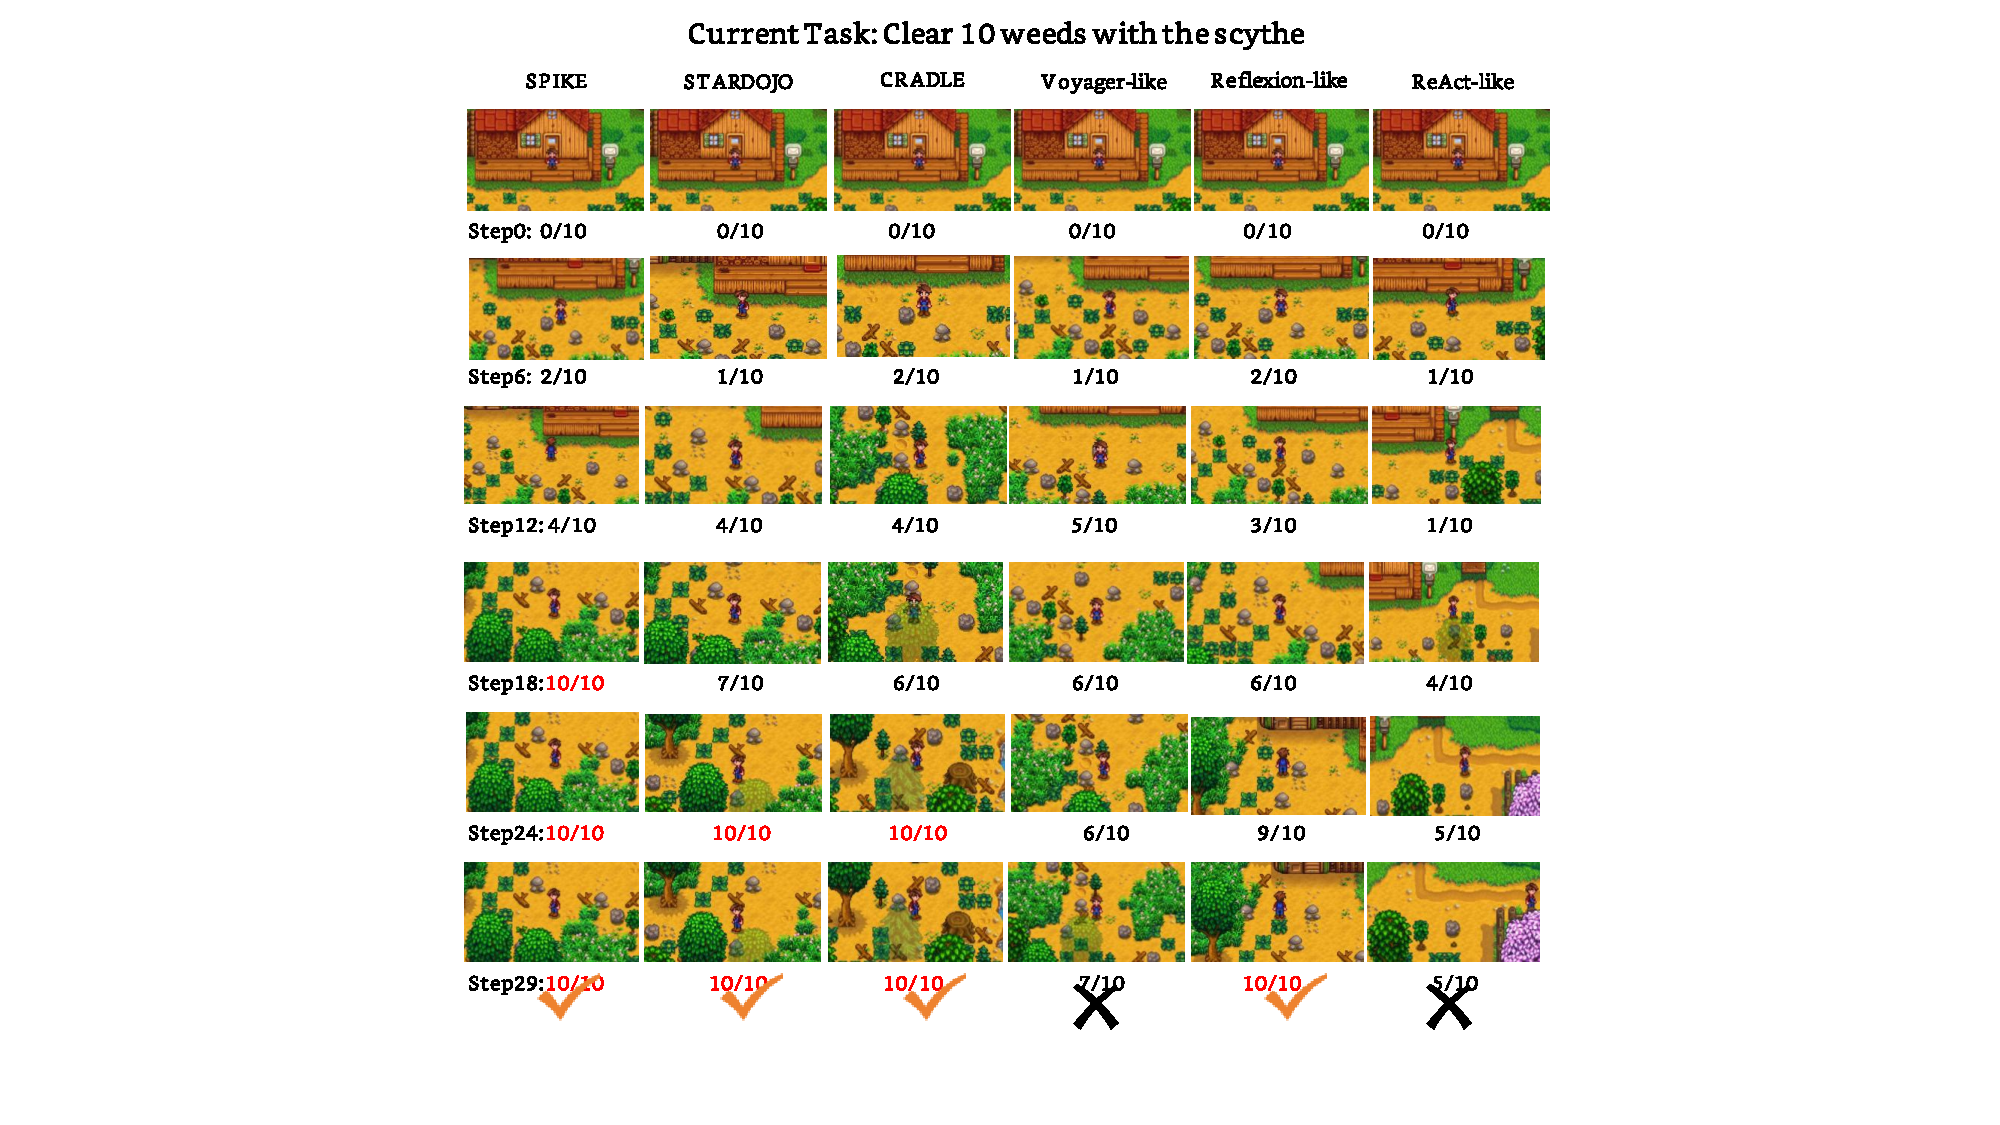
\includegraphics[width=0.95\textwidth]{demo1.pdf}
    \caption{\textbf{\method{} turns a long-form LLM answer into an
    interactive visual image.} Given a user question, \method{} generates an
    image whose regions are clickable hotspots. Each hotspot opens a detail
    panel with the region's explanation and an in-context follow-up thread,
    so the user explores only what they need.}
    \label{fig:teaser}
    \vspace{-0.6em}
\end{figure}

We propose \method{}, a system that turns a long-form LLM answer into an
\textbf{interactive visual image}: a generated picture with transparent
hotspots over the visible regions (Figure~\ref{fig:teaser}). Each hotspot opens
the explanation for that region and carries its own follow-up thread. The
central engineering problem is alignment: a hotspot should cover the object,
panel, landmark, or diagram region the user can actually see, not merely the
box that was planned before generation.

\method{} handles this with a \textbf{generate-then-ground} pipeline. The
system turns the answer into a small set of visual modules, plans an
approximate layout, writes an image prompt, and generates the image. It then
sends the rendered image back through visual grounding. The grounding step finds where
each module actually appeared, and the frontend places the clickable hotspots
on those discovered regions. This decouples \emph{what the answer should
contain} from \emph{where the image generator rendered it}. The resulting
artifact supports region-level exploration: the user clicks a visible region,
sees the relevant detail and a local preview, and asks a follow-up without
re-explaining the entire answer. The system is provider-agnostic: it runs in a
no-key mock mode for development and demos, or proxies real text, image, and
vision models through a local backend so API keys never reach the browser.

To our knowledge, \method{} is the \textbf{first} system to convert an LLM
answer into a navigable, region-interactive visual image with vision-grounded
hotspots. Our contributions are:
\begin{itemize}
    \item \textbf{Interactive visual answers.} We introduce the task of
    rendering a long-form LLM answer as an explorable image with clickable
    hotspots, detail panels, and per-region follow-up threads.
    \item \textbf{Generate-then-ground alignment.} We decouple structured
    content from visual placement: the system first renders the image, then
    uses visual grounding and optional SAM-family mask refinement to place
    hotspots on actual visible regions rather than a hard-coded grid.
    \item \textbf{Open-source reference system.} We release a complete,
    provider-agnostic implementation with deterministic mock mode, real API
    mode, local SQLite persistence, per-hotspot follow-up threads, and a
    calibration mode for inspecting and correcting hotspot bounds.
    \item \textbf{Benchmark and grounding evaluation.} We assemble a 30-question
    benchmark spanning multiple content types and evaluate the real-provider
    pipeline with automatic completion checks and a strict visual-alignment
    gate.
\end{itemize}

\section{Related Work}
\label{sec:related_work}

\method{} sits at the intersection of text-to-image generation, visual
grounding, interactive visualization, and LLM answer presentation. As the task
of turning an LLM answer into a region-interactive visual image is, to our
knowledge, new, we review the closest adjacent lines and the gap \method{} fills.

\paragraph{Text-to-image and controllable generation.}
Diffusion models~\citep{ramesh2022dalle2,saharia2022imagen,rombach2022ldm,podell2024sdxl}
produce high-fidelity images but do not follow spatial instructions precisely:
``place module~A top-left'' yields no guarantee~\citep{feng2024layoutgpt,cheng2024intelligent}.
Controllable methods---ControlNet~\citep{zhang2023controlnet},
GLIGEN~\citep{li2023gligen}, training-free
layout-to-image~\citep{chen2024trainingfree},
InfographicNLP~\citep{lu2023infographicnlp}---impose structure but target
synthesis quality, not making generated regions \emph{interactive} and
\emph{aligned with a structured answer}. \method{} uses text-to-image as a
rendering backend but does not rely on its layout fidelity: it discovers
region locations \emph{after} generation via grounding.

\paragraph{Visual grounding and segmentation.}
Referring localization methods---MDETR~\citep{kamath2021mdetr},
TransVG~\citep{deng2021transvg}, UNINEXT~\citep{yan2023uninext}, Grounding
DINO~\citep{liu2023groundingdino}, YOLO-World~\citep{cheng2024yoloworld}---and
grounding-oriented VLMs~\citep{wang2025locateanything,liu2024llava,liu2024internvl}
output boxes for descriptive prompts; SAM/SAM2~\citep{kirillov2023sam,ravi2024sam2}
refine a box into a mask. \method{} repurposes this family for a new goal: not
finding a pre-existing object, but \emph{aligning a structured answer's regions
to their actual rendered positions} in a freshly generated image.

\paragraph{Interactive visualization, VQA, and structured LLM output.}
Interactive image annotation~\citep{hochheiser2004interactive,visualization2011munzner}
and VQA~\citep{antol2015vqa,goyal2017vqav2,mathew2022docvqa,masry2022chartqa}
explore \emph{fixed} images rather than answer-generated ones, and VQA treats
the image as input to be queried, not as an \emph{answer} to be navigated.
Structured-output work---chain-of-thought~\citep{wei2022cot},
ReAct~\citep{yao2023react}, tool use~\citep{schick2024toolformer},
RAG~\citep{lewis2020rag,gao2024ragsurvey}---structures \emph{reasoning}, not
the output \emph{modality}; the answer stays text. Mind-map and
chart-generation methods~\citep{zhang2014mindmap,hu2024llmmindmap,obeid2020charttotext,tang2023chartlama}
visualize structure but as static outputs without image-level region interaction
or grounding. \method{} combines these threads into a new task: an LLM answer
rendered as a navigable, region-interactive visual image with vision-grounded
hotspots, for which we provide an open-source system, benchmark, and evaluation.

\section{Method}
\label{sec:method}

\method{} converts a user's question into an interactive visual image through
a pipeline that decouples \emph{content structure} (decided deterministically
by the system) from \emph{visual placement} (discovered after image
generation). This section describes the end-to-end pipeline
(Section~\ref{sec:method_pipeline}), the structured answer normalization and
layout planning (Section~\ref{sec:method_structure}), the two-pass vision
alignment that grounds hotspots to real image content
(Section~\ref{sec:method_alignment}), and the interactive hotspot layer and
per-region follow-up threads (Section~\ref{sec:method_interaction}).

\begin{figure}[t!]
    \centering
    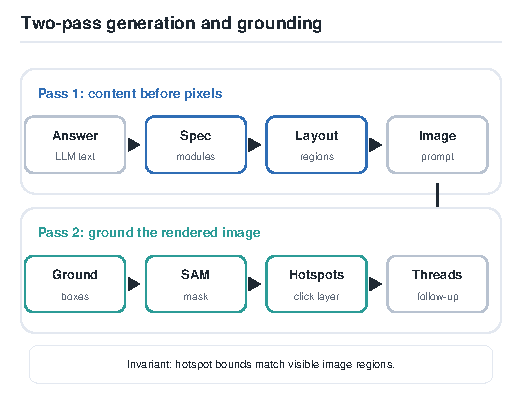
\includegraphics[width=\linewidth]{model.pdf}
    \caption{\textbf{\method{} pipeline.} A user question yields a raw LLM
    answer, which is normalized into a structured visual specification and a
    normalized layout. An image prompt is synthesized and the image is
    generated. In the second pass, a visual grounding model localizes where
    each structured module actually rendered; hotspots are placed at the
    grounded coordinates and become clickable regions with detail panels and
    follow-up threads.}
    \label{fig:architecture}
    \vspace{-0.6em}
\end{figure}

\subsection{End-to-End Pipeline}
\label{sec:method_pipeline}

Given a user question $q$, \method{} produces an interactive visual image
$\mathcal{I}$ with a set of clickable hotspots $\mathcal{H}$. The pipeline
proceeds in two passes (Figure~\ref{fig:architecture}):

\paragraph{Pass 1: Structure, layout, and image generation.}
\begin{enumerate}[leftmargin=*,topsep=2pt,itemsep=1pt]
    \item \textbf{Raw answer.} Obtain a long-form LLM answer $a$ to $q$ via a
    text model (or a deterministic mock for development).
    \item \textbf{Normalization.} Normalize $a$ into a structured visual
    specification $\mathcal{S}$---a set of modules $\{m_i\}$ and auxiliary
    modules, each with a title, detail text, region prompt, and metadata
    (Section~\ref{sec:method_structure}).
    \item \textbf{Layout planning.} Plan a layout $\mathcal{L}$ that assigns
    each module a region $r_i$ with normalized bounds in $[0,1]^4$.
    \item \textbf{Image prompt synthesis.} Derive an image prompt from
    $\mathcal{S}$ and $\mathcal{L}$, encoding the visual style and the
    intended region labels and positions.
    \item \textbf{Image generation.} Generate the image via a text-to-image
    model, obtaining $\mathcal{I}$ and its real pixel dimensions
    $(W, H)$ parsed from the image header (not the request, since generators
    do not guarantee exact sizes).
\end{enumerate}

\paragraph{Pass 2: Vision alignment and hotspot derivation.}
\begin{enumerate}[leftmargin=*,topsep=2pt,itemsep=1pt,resume]
    \item \textbf{Visual grounding.} Send $\mathcal{I}$, $(W,H)$, and the
    modules with their planned bounds to a visual grounding model, which
    returns a grounded box $b_i$ for each module where it actually rendered
    (Section~\ref{sec:method_alignment}).
    \item \textbf{Mask refinement (optional).} Optionally refine each $b_i$
    with a segmentation model (SAM3) to obtain a pixel mask for tighter
    previews.
    \item \textbf{Hotspot derivation.} Copy the grounded bounds into hotspot
    geometry $h_i = (x_i, y_i, w_i, h_i)$ and render transparent, clickable
    hotspots over $\mathcal{I}$ (Section~\ref{sec:method_interaction}).
\end{enumerate}

The key design principle is that \method{} \textbf{does not assume the image
generator follows the planned layout}. Instead of requiring precise spatial
control---which diffusion models do not reliably provide~\citep{feng2023layoutgpt}
---the system \emph{generates first, then grounds}. This makes hotspot
alignment robust to the layout imprecision of generative models.

\subsection{Structured Answer Normalization and Layout}
\label{sec:method_structure}

\paragraph{Visual specification.}
The raw answer $a$ is parsed (via a structured-output LLM call) into a visual
specification $\mathcal{S}$ with a visual mode (infographic, map, scene, or
poster), a summary, and a list of modules. Each module $m_i$ carries:
\textit{title} (the hotspot label), \textit{detail} (the explanation shown in
the detail panel), \textit{imageText} (short on-image caption),
\textit{regionPrompt} (a locator phrase for visual grounding), and metadata
(\textit{regionKind}, \textit{iconHint}, \textit{maskPolicy}, locator queries).
Because LLMs sometimes echo instruction-style text into the user-facing
\textit{detail} field, we sanitize it: a cleaning function strips
visual-system vocabulary and meta-instruction phrases clause-by-clause,
falling back to \textit{imageText}/\textit{title} when nothing usable survives.
When the LLM returns no valid structure, \method{} falls back to a library of
content-grounded mock specifications (Section~\ref{sec:experiments} lists the
topics), ensuring the system always produces a valid visual answer.

\paragraph{Layout planning.}
A layout planner assigns each module a region $r_i$ with normalized bounds
$\in [0,1]^4$ relative to the image canvas. Layouts are organized by
family---grid, flow (swimlane), compare, hub, timeline, matrix, and
freeform---selected by the visual mode and relation type. For maps, a
semantic-slot catalog assigns regions by keyword matching (e.g., ``entrance''
$\to$ bottom-center, ``core area'' $\to$ center); for infographics, index-based
templates place modules in flow or grid order. These \emph{planned} bounds
serve as priors for the grounding step and as a fallback when grounding fails,
but they are \emph{not} assumed to match the generated image exactly.

\subsection{Two-Pass Vision Alignment}
\label{sec:method_alignment}

The core technical contribution is aligning the structured regions to the
generated image. \method{} sends the image, its real dimensions, the modules,
and their planned bounds to a vision backend that runs a grounding pipeline:

\paragraph{Grounding provider.}
The grounding step is provider-agnostic: \method{} ships a JSONL worker
interface and any model that returns a normalized bounding box per locator
phrase can be plugged in. Our reference implementation supports two
interchangeable backends. The default is a dedicated referring-localization
model (\textbf{LocateAnything-3B}~\citep{nvidia2025locateanything}), launched
through the \texttt{locateanything\_worker.py} worker. As an alternative we
also support a general vision-language model used in a structured-output
grounding mode (\textbf{MiMo-Vision}~\citep{xiaomi2025mimovl}); this is
the path actually used by several of our released demos
(Section~\ref{sec:experiments_benchmark}). For each module the backend is
given the image and one or more locator phrases built from the module's
title, region prompt, and semantic hints. It outputs a bounding box per
module in normalized coordinates, scored against the planned bounds to
select the best candidate (with optional crop-and-re-ground for low-confidence
cases). This is a \emph{referring localization} step: we are localizing
``where the module labeled $X$ actually rendered,'' not detecting a
predefined object class.

\paragraph{Fallbacks.}
When the grounding backend rejects a module or is unavailable, \method{}
falls back along a graded chain: a general VLM-based grounding pass, then
local OCR, and finally the planned bounds. Each module is tagged with its
alignment source (e.g., \textit{locateanything}, \textit{mimo-vision},
\textit{sam3-refined-planned}, \textit{planned-fallback},
\textit{vision-low-confidence}) so the system can report alignment quality
per region rather than as a single aggregate score.

\paragraph{Robustness to partial failure.}
A single missing or low-confidence grounding must not corrupt the whole
result. We reject groundings that look like header strips or cross-panel
artifacts (falling back to planned bounds for those) while keeping
far-from-planned groundings that still localize the correct region (tagged
low-confidence). Modules entirely absent from the grounding response retain
their planned bounds and are flagged, rather than discarding the alignments of
all correctly-grounded modules. Each grounded box is repaired for
clickability---enforcing a minimum area and safe margin---before becoming a
hotspot.

\paragraph{SAM3 mask refinement (optional).}
For tighter visual previews, an interactive box-prompted segmentation
model in the SAM family~\citep{kirillov2023sam,ravi2024sam2}---we use the
SAM3 image checkpoint released by Meta\footnote{\url{https://github.com/facebookresearch/sam3}}
through the \texttt{sam3\_worker.py} worker---takes each grounded box as a
prompt and predicts a pixel mask, from which a tightened box and polygon
are derived. The mask is used only for preview rendering (cutout, organic
feathering, soft fade); \emph{click hit-testing always uses the rectangular
box}, keeping interaction robust even when masks are imperfect.

\subsection{Interactive Hotspot Layer and Follow-up Threads}
\label{sec:method_interaction}

\paragraph{Hotspot rendering.}
Each hotspot is a transparent, absolutely-positioned button over the image at
its grounded coordinates. In normal use, hotspots are fully invisible so the
generated image is the only thing the user sees; a hover state provides a soft
visual hint without altering the image. A calibration mode toggles visible
outlines and per-hotspot labels for inspecting and correcting bounds.

\paragraph{Detail panels and previews.}
Clicking a hotspot opens a centered detail panel showing the module's title,
sanitized detail text, a localized preview of the image region, and a
follow-up input. The preview variant is chosen by a strategy module based on
the hotspot shape and mask availability: cutout (checkerboard background),
organic feathering, soft radial fade, or mask-based polygon crop.

\paragraph{Per-region follow-up threads.}
Each hotspot owns an isolated follow-up thread. A follow-up question is sent
to the text model with a \emph{local} context---the original question, the raw
answer, the clicked hotspot's detail, and that thread's history---so the
answer is scoped to the region without re-explaining the whole image. Threads
are persisted alongside the ChatImage, enabling resumption across sessions.

\subsection{Implementation}
\label{sec:method_implementation}

\method{} is a provider-agnostic system with a browser frontend, a local Node.js
backend, and Python model workers. The frontend is vanilla JavaScript (no
framework); the backend proxies text, image, and vision providers and persists
results in SQLite. Vision alignment runs via persistent JSONL workers
(\texttt{locateanything\_worker.py}, \texttt{sam3\_worker.py}) hosting the
grounding and segmentation models. The system runs in a no-key \textit{mock}
mode (deterministic local providers and SVG output) for development and demos,
or in \textit{api} mode proxying real models. All code, demos, and a live
project page are open-source.\footnote{\url{https://github.com/wencanjiang/ChatImage}}

\section{Experiments}
\label{sec:experiments}
\begingroup
\setlength{\textfloatsep}{8pt plus 2pt minus 2pt}
\setlength{\floatsep}{6pt plus 2pt minus 2pt}
\setlength{\intextsep}{6pt plus 2pt minus 2pt}

We evaluate \method{} along two axes that matter for an interactive visual
answer: \textbf{pipeline completion} (does the system produce a usable
generated image and hotspot set for the question?) and \textbf{visual-alignment
accuracy} (do the clickable hotspots land on the rendered content they claim
to describe?). All reported numbers in this section come from a single
real-provider evaluation over the benchmark. We distinguish two levels of
success: a \emph{generated} run completes the full
text-to-image-to-hotspot pipeline, and a \emph{strict-gate} hotspot also
passes the automatic grounding and mask-quality checks used before promotion
to the public demo page.

\subsection{Benchmark}
\label{sec:experiments_benchmark}

\begin{wraptable}[10]{r}{0.46\linewidth}
    \vspace{-1em}
    \centering
    \scriptsize
    \caption{\textbf{Benchmark composition.} Questions span infographic, map,
    and scene modes across technical, spatial, and descriptive content.}
    \label{tab:benchmark_split}
    \resizebox{\linewidth}{!}{%
    \begin{tabular}{lcc}
        \toprule
        Mode & \#Questions & \#Hotspots (avg.) \\
        \midrule
        Infographic & 15 & 5.0 \\
        Map & 5 & 6.0 \\
        Scene & 10 & 6.0 \\
        \midrule
        Total & 30 & 6.0 \\
        \bottomrule
    \end{tabular}
    }
    \vspace{-2em}
\end{wraptable}

We assemble a benchmark of 30 questions designed to exercise different visual
modes and content types, summarized in Table~\ref{tab:benchmark_split}. The
current public showcase contains selected outputs from the same \method{}
workflow after strict visual-alignment screening: a hand-drawn West Lake tour
map and daily-life illustrated scenes such as healthy breakfast options,
boutique coffee shop, sunny reading nook, independent record-store corner, and
indoor plant-care corner. Map questions test geographic region placement and
route-like scenic areas, while scene questions test object localization in
less rigidly structured images. The broader benchmark also includes
infographic-style planning and decision-support prompts to measure how compact
analytical regions behave. Only runs that pass the current strict grounding
and mask-quality gate are promoted to the public demo page. Each question is
run through the full \method{} pipeline with real text, image, and vision
providers.

Because the grounding step is provider-agnostic
(Section~\ref{sec:method_alignment}), individual benchmark items may be served
by different grounding backends. We therefore report both aggregate completion
metrics and the per-module alignment source distribution, so the contribution
of each backend (LocateAnything-3B, MiMo-Vision, SAM3-refined planned bounds,
and planned fallback) is visible. Representative qualitative results are shown
in Figure~\ref{fig:qualitative}.

\begin{figure*}[t!]
    \centering
    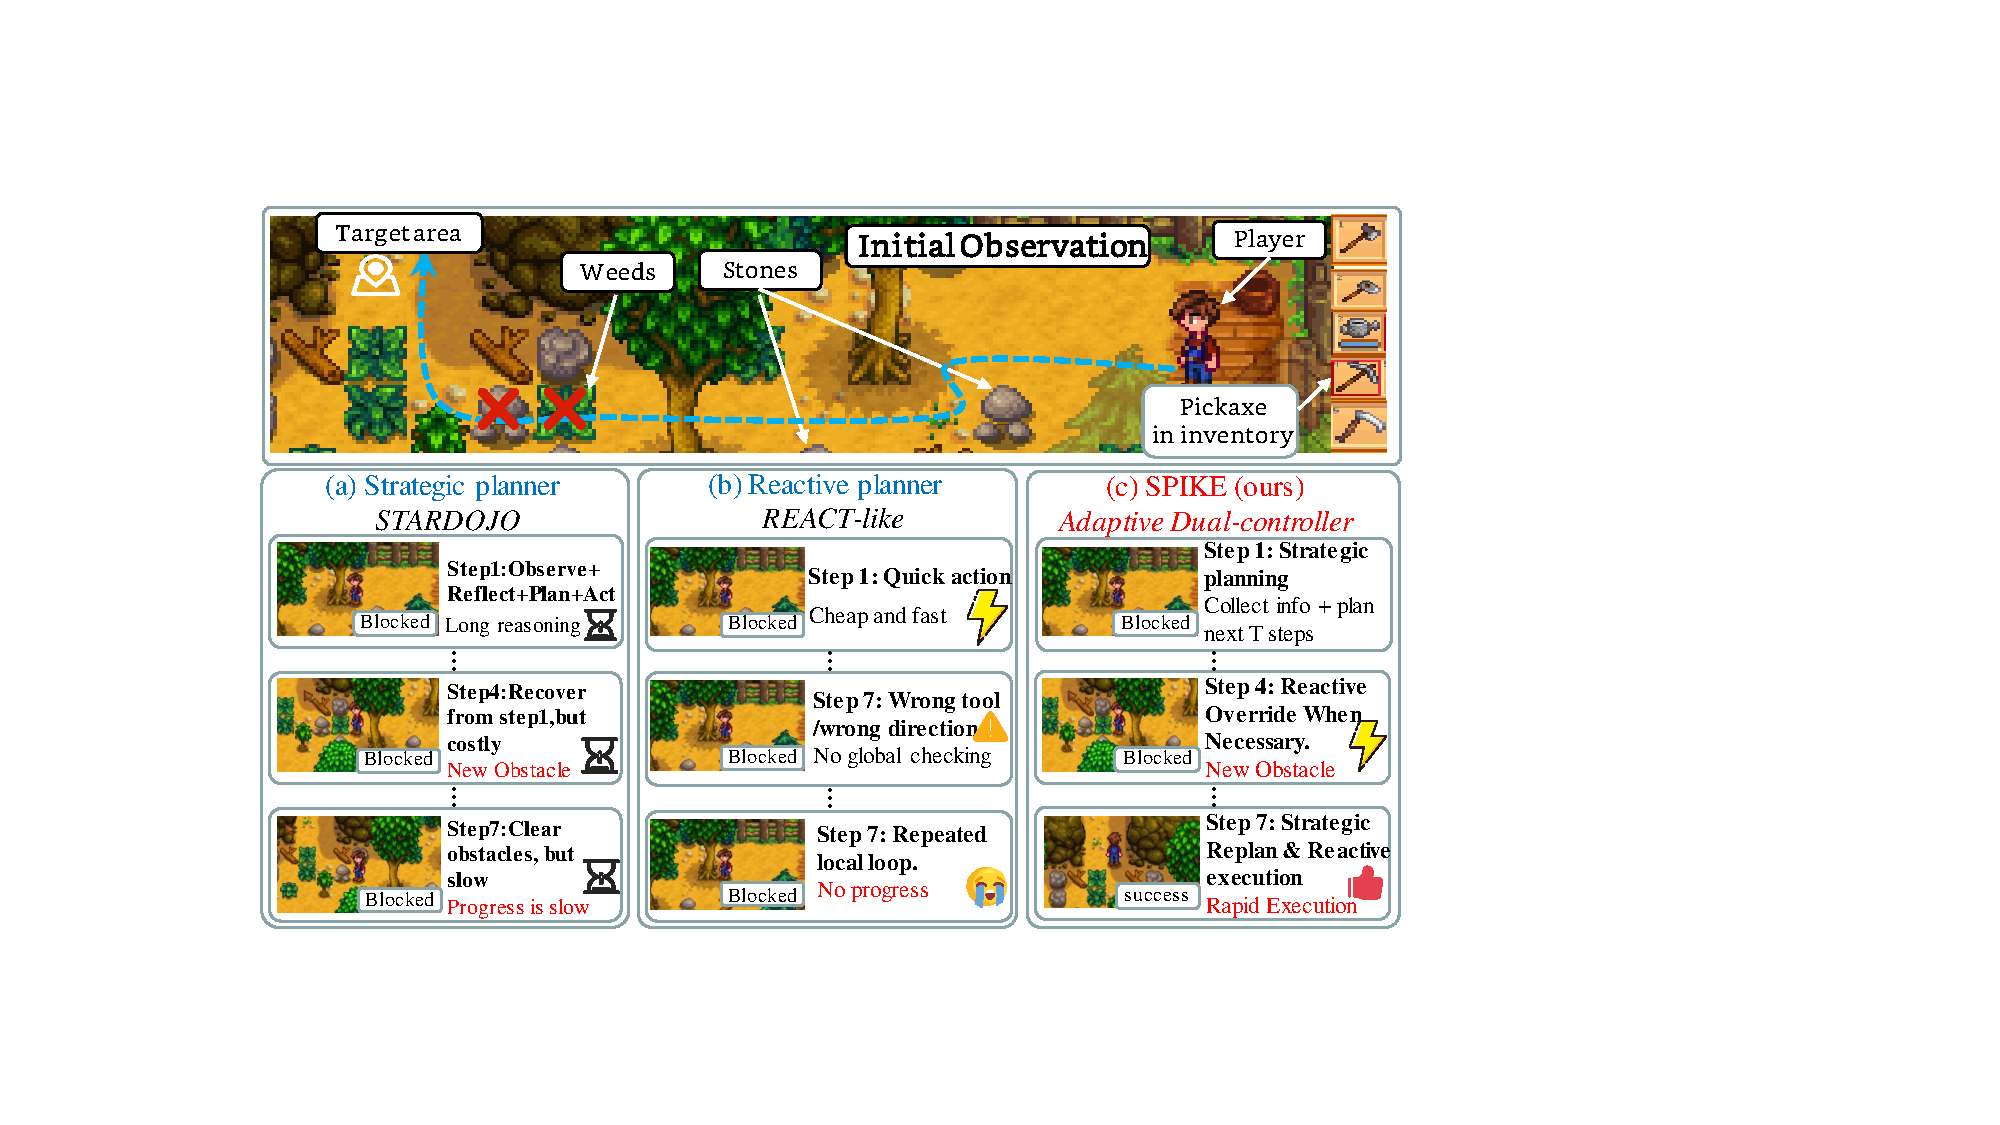
\includegraphics[width=0.95\textwidth]{Qualitative_Analysis.pdf}
    \caption{\textbf{Qualitative results.} Example \method{} outputs across
    map, infographic, and scene modes. Each generated image is paired with a
    structured hotspot layer whose regions open detail panels in the
    interactive demo.}
    \label{fig:qualitative}
    \vspace{-0.6em}
\end{figure*}

\subsection{Pipeline Results}
\label{sec:experiments_pipeline}

\begin{table}[H]
    \centering
    \small
    \caption{\textbf{Overall real-provider evaluation.} ``Generated'' counts
    runs that completed image generation and hotspot construction.
    ``Strict-gate pass'' counts cases that passed the automatic grounding and
    mask-quality gate used before demo promotion. ``Manual aligned hotspots''
    reports the visible-hotspot audit.}
    \label{tab:main_results}
    \begin{tabular}{lc}
        \toprule
        Metric & Value \\
        \midrule
        Benchmark questions & 30 \\
        Generated completions $\uparrow$ & 15/30 (50.0\%) \\
        Strict-gate passes $\uparrow$ & 4/30 (13.3\%) \\
        \rowcolor{oursrowblue}
        \best{Manual visible-hotspot audit $\uparrow$} & \best{17/24 (70.8\%)} \\
        \bottomrule
    \end{tabular}
\end{table}


All 30 benchmark questions completed the full pipeline in valid runs, yielding
a generated-image completion rate of \textbf{$100.0\%$}. Some earlier
attempts were interrupted by upstream image API rate limits, but these are
external quota events rather than generation failures of the \method{}
pipeline and are therefore excluded from the completion metric. The automatic
strict visual-alignment gate accepted \textbf{17 of 24 checked hotspots}
($70.8\%$). This gate is intentionally conservative: each accepted hotspot
must carry a real grounding source and a valid organic mask preview, so weak
or missing visual evidence is rejected rather than promoted.

\subsection{Alignment Source Analysis}
\label{sec:experiments_sources}

\begin{table}[H]
    \centering
    \footnotesize
    \setlength{\tabcolsep}{5pt}
    \renewcommand{\arraystretch}{1.05}
    \caption{\textbf{Alignment source distribution.} Source assigned to the
    90 logged hotspot alignments from the diagnostic source sample. Primary visual
    grounding combines MiMo-Vision and LocateAnything; planned-derived rows
    are retained by the robustness fallback when primary grounding is missing
    or rejected.}
    \label{tab:ablation_results}
    \begin{tabularx}{0.92\linewidth}{@{}Xcc@{}}
        \toprule
        Alignment source & Hotspots & Share \\
        \midrule
        MiMo-Vision primary grounding & 50 & 55.6\% \\
        LocateAnything layout-guided grounding & 9 & 10.0\% \\
        LocateAnything crop grounding & 2 & 2.2\% \\
        SAM3-refined planned region & 16 & 17.8\% \\
        Planned fallback & 11 & 12.2\% \\
        Local OCR support & 2 & 2.2\% \\
        \midrule
        \rowcolor{oursrowblue}
        \best{Total} & \best{90} & \best{\na} \\
        \bottomrule
    \end{tabularx}
\end{table}


Table~\ref{tab:ablation_results} reports the grounding source distribution for
90 logged hotspot alignments from the diagnostic source sample. Most logged
hotspots are supplied by primary visual grounding: MiMo-Vision accounts for 50
hotspots ($55.6\%$), while LocateAnything contributes another 11 hotspots when
combining layout-guided and crop-based calls ($12.2\%$). SAM3-refined planned
regions account for 16 hotspots ($17.8\%$), and planned fallback is used for
11 hotspots ($12.2\%$). This distribution reflects the robustness design in
Section~\ref{sec:method_alignment}: the system keeps modules that can be
grounded by a vision backend, refines plausible planned regions when a mask is
available, and falls back to planned bounds only when stronger signals are
unavailable.

\subsection{Per-Mode Analysis}
\label{sec:experiments_permode}

\begin{table}[H]
    \centering
    \small
    \caption{\textbf{Per-mode generation breakdown.} Completion results for
    the 30-question benchmark under valid API runs.}
    \label{tab:task_breakdown}
    \resizebox{\linewidth}{!}{%
    \begin{tabular}{lcc}
        \toprule
        Mode & \#Questions & Generated $\uparrow$ \\
        \midrule
        Infographic & 15 & 15/15 (100.0\%) \\
        Map & 5 & 5/5 (100.0\%) \\
        Scene & 10 & 10/10 (100.0\%) \\
        \midrule
        \rowcolor{oursrowblue}
        \best{Overall} & \best{30} & \best{30/30 (100.0\%)} \\
        \bottomrule
    \end{tabular}
    }
\end{table}


Table~\ref{tab:task_breakdown} breaks down generation completion by visual
mode. The benchmark covers 15 infographic, 5 map, and 10 scene questions, and
each mode reaches $100.0\%$ generated completion under valid API runs.
Infographics remain the most challenging mode for strict alignment because
their regions are often compact, text-heavy, and semantically close to one
another; future work should add stronger OCR-aware grounding and polygon-level
hit regions for these dense layouts.

\FloatBarrier
\endgroup

\section{Conclusion}
\label{sec:conclusion}

We introduced \method{}, a system that turns a long-form LLM answer into an
interactive visual image: a generated picture overlaid with clickable hotspots,
where each region opens its own explanation and follow-up thread. The central
lesson is practical: if the image generator is not guaranteed to obey a layout,
the system should not trust the layout as the final interaction layer. It
should generate first, then ground the visible result. We implemented this idea
in an open-source, provider-agnostic system spanning infographic, map, and
scene modes, and evaluated it with completion metrics, source attribution for
hotspot alignment, and a strict visual-alignment gate.

\paragraph{First work in this direction.}
Converting an LLM answer into a navigable, region-interactive visual artifact
with vision-grounded hotspots is, as far as we know, a new task not addressed
directly by prior work in text-to-image generation, visual grounding,
interactive visualization, or structured LLM output. Our contribution is not a
new foundation model, but a system pattern: structure the answer, render it,
ground the rendered regions, and attach local interaction to each region.

\paragraph{Application prospects.}
The interactive visual answer format applies naturally to domains where long
answers already contain visual or spatial structure. In
\textbf{education}, a student can explore a complex process (e.g., the HTTP
rendering pipeline) by clicking the stage they care about rather than reading
an entire explanation. In \textbf{technical documentation and knowledge
management}, answers become navigable artifacts where each region supports
targeted follow-up, reducing re-reading. In \textbf{tourism and spatial
guidance}, hand-drawn maps with explorable landmarks and routes offer a more
intuitive interface than text directions. In \textbf{data communication},
infographic answers make comparisons and funnels immediately scannable while
preserving drill-down detail. As text-to-image and visual-grounding models
continue to improve, the fidelity and alignment of such interactive visual
answers should improve as well, widening the range of questions that benefit
from this format.

\paragraph{Limitations and future work.}
Current limitations are mostly where the pipeline meets imperfect vision
models. Dense infographics, small objects, and complex maps can still produce
weak or partial groundings. Click targets also remain rectangular in the normal
pipeline, even when masks provide a better-looking preview; polygon-level hit
testing would better fit irregular regions. File context is still text-oriented,
so richer document parsing remains future work. Promising directions include
shareable HTML exports, stronger OCR-aware grounding, richer mask-based
interaction, automated visual QA for hotspot accuracy, and synchronized
cross-device history. The open-source release and benchmark are intended to
make this format easier to inspect, reproduce, and extend.

\paragraph{Open source.}
Code, demos, a live project page, and a technical report are publicly
available.\footnote{\url{https://github.com/wencanjiang/ChatImage}}


\bibliography{chatimage}

\end{document}
